\chapter{Introduction}
Performance of operating system is crucial, because it can significantly affect all the applications running above it.
When a regression in new version occurs, business applications can be even financially affected.

Scheduler was simple. Multi-core CPUs made the scheduler little more complex, but those complications were tuned through time.
Next milestone was introduction of multi-CPU machines with separated memory for each physical unit.

Compared to functional testing, performance isn't evaluated as true/false result, but relative change to previous measurement.
Due to this complexity is hard to use common tools for inspecting performance.
The biggest regression in scheduler doesn't hide in uneffective code, but in wrong placement of processes to cores and it's queues.

The usual testing method is simulating load simmilar to real usage.
To achieve this there are many benchmarks targetting different types of load, usually many parallel process, sometimes communicating between each other.

Good performance tests usually create great amount of data, which is required to be processed, aggregaed and visualised.

\chapter{Linux process scheduling}

\section{Completely Fair Scheduler}
Completely Fair Scheduler is process scheduler which replaced the O(1) scheduler
in version 2.6.23 of Linux kernel. It orders processes using red-black tree where it
chooses process with the lowest spent execution time.
\texttt{https://en.wikipedia.org/wiki/Completely\_Fair\_Scheduler}

Single processor is simple, problems come with NUMA nodes. Switching between
nodes or reading from another is expensive.
Another problem is when scheduler leaves cores idle, even where there are
runnable threads waiting.


\chapter{Performance measurement}
A basic way to measure performance of system is benchmark. They return some numbers representing throughput of system, but can't tell more about the system behavior.
To get a better insight on the system, there are many performance analysis tools to observe cpu and memory utilization, location of processes on cores or their time out of cpu.
\texttt{http://www.brendangregg.com/activebenchmarking.html}

\section{Benchmarks}

\subsection{NAS Parallel Benchmarks}
NAS Parallel Benchmarks is a set of small programs to help evaluate performance of parallel supercomputers.
\texttt{https://www.nas.nasa.gov/publications/npb.html}

NAS Parallel consists of small programs performing highly parallel computations.
Can be run on variable number of threads. Has different sizes of workload to fit
machines with wide range of performance.
It's written in languages C and Fortran.

\subsection{SPECjbb2005}
Java Business Benchmark behaves as a server-side Java application. It is primarily focused on measuring performance of Java implementation, but also reflects performance of operating system and cpu itself.
It models system of wholesale company as a multitier application. The benchmark
itself creates the load, measures the throughput and also generates simple
report in HTML and raw text formats.

The main output value is \emph{throughput} in units called \emph{SPECjbb2005
  bops} \footnote{Business operations per second}.
In case of using more JVM instances, there is a second unit called SPECjbb2005
bops/JVM representing average throughput of single JVM\footnote{Java virtual machine} instance.
Another collected metric is memory comsumption, which isn't that useful in
scheduler performance monitoring.

\subsection{LINPACK benchmark}
LINPACK Benchmark comes from LINPACK package, wich was used to solve systems of linear equations in single or double precision.

\subsection{Stream benchmark}

\section{Performance analysis tools}

\subsection{time}
Simple command, that can measure resource usage. Usually it's used to measure
running time of process.

It isn't bash builtin, but programm, that must be usually called from /usr/bin/time.

\subsection{ps}
This command lists current processes with information about them. In
\texttt{PSR} and \texttt{NUMA} column are useful informations of CPU and NUMA
node number, where is the process running.

\subsection{mpstat}

\subsection{turbostat}
This tool provides measuring of CPU usage and mainly its frequency.

\subsection{perf}


\chapter{Storing the results}
Benchmarks usually generate long human-readable output in text or even HTML
format. This is useful when analyzing single report. In the output are details
of the test run itself, simple resource usage or success of result validation.
However, the amount of result starts to rise with repeated runs, different
amount of instances and new versions kernels.

For the comparison of performance results, it is usually enough the number
representing throughput or time of each benchmark run. Those numbers can be
preprocessed from the benchmark output files to a format more suitable for quick
accesing required data.

\section{XML files}
XML is markup language, that can store heterogeneous data in tree structure.
However, the main feature of this format is human-readability. Even with the
inefficient storage of numerical data and repetition of tag and attribute names,
it allows user to quicky see the numbers without any processing of the data.

\section{Database}


\chapter{Displaying the results}

\section{Heatmaps}

\section{Boxplots}
Boxplot is method for displaying statistical properties of data groups. The
usually displayed values are minimum, 1\textsuperscript{st} quartile, median, 3\textsuperscript{rd} quartile and maximum.
This feature is useful to visualize accuaracy and reliability of measurement.
Then it's easier to distinguish performance regression from noise.

\begin{figure}
  \centering
  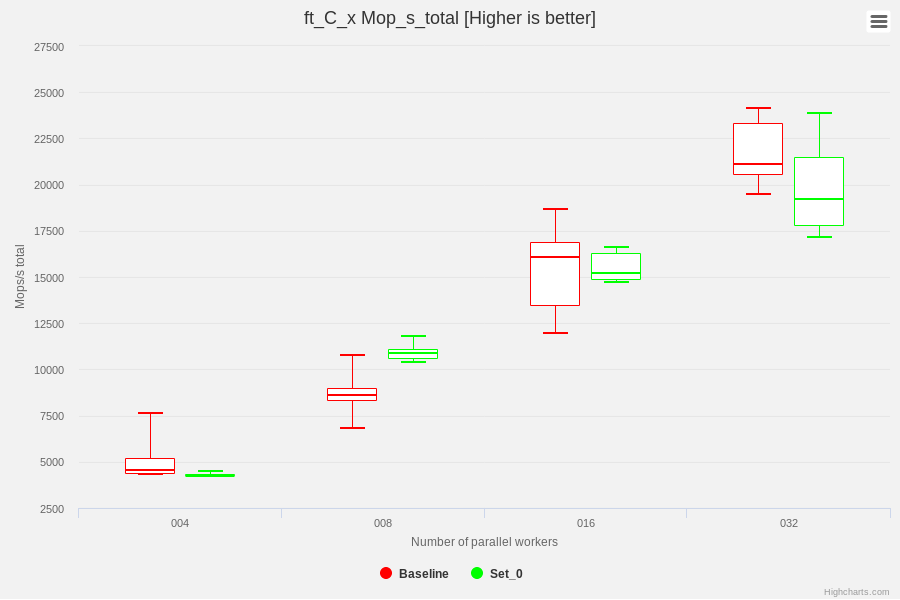
\includegraphics[width=12cm]{obrazky-figures/boxplot}
  \caption{Example of boxplot showing Mops of NAS benchmark with different
    number of threads}
\end{figure}


\chapter{Timelines}


\chapter{Automatic evaluation}


\chapter{Future work}


\chapter{Notes}
\begin{verbatim}
Linux scheduler
    CFS
    numa planning
        not easy for scheduler
        manual pinning option
            numactl
        group imbalance bug
    tune profiles
        focus on throughput or latency
Performance
    performance isn't simple pass/fail
    comparison of baseline and target kernel
    running just benchmark is waste of testing potential, it's good to collect more data
        http://www.brendangregg.com/activebenchmarking.html
    provisioning of machines with Beaker
    collecting system load data
        mpstat
            usage of every cpu
        numastat
        numatop
            usage of cpu and memory on each node
        ps
            psr and numa column
            cpu time
        time
            total, user and system time spent
        turbostat
        perf stat
        lstopo for hardware schema image
        free
    benchmarks
        specjbb2005
        specjvm2008
        nas parallel
        linpack benchmark
        stream (memory throughput)
        specjbb2015 - not stable
        hackbench - not tried yet
    scenarios
        variable number of benchmark instances
        with and without pinning processes to specific numa nodes
    result storing
        preprocessing to xml
        storing to database
        aggregating results
        computing statistical data
    plotting
        lstopo for plotting hardware topology
        bargraphs to show inaccuaracy
            operations per second (runtime of benchmark)
            time out of cpu
        detailed comparsion of two results
        timeline with many results over longer period of time
        heatmaps for core usage over time
            http://www.brendangregg.com/HeatMaps/utilization.html
        graph of process migration between numa nodes
Timelines
    analysis
    used technologies
    desing
    implementation
    output
Automatic regression detection
    motivation
    marking data
    preprocessing for classificator
    methods
        linear logistic regression
        decision trees
    evaluation
\end{verbatim}

\chapter{Specification}
\begin{enumerate}
\item Get acquainted with the existing methods for measuring performance of the Linux kernel scheduler and with means of storing of benchmarks results for further processing.
\item Study possible ways of processing these results with a focus on graphic interpretation and on methods for detection of performance degradation.
\item Design and implement a method for efficient graphic interpretation of long-term measurements.
\item Design and implement a method for automatic detection of performance regression.
\item Demonstrate the functionality of your implementation on at least two versions of the Linux kernel.
\item Evaluate the obtained results and discuss possibilities of further development of the project, especially of the automatic detection of performance regression.
\end{enumerate}

Literature:
\begin{itemize}
\item Lozi, Jean-Pierre, et al. "The Linux scheduler: a decade of wasted cores." Proceedings of the Eleventh European Conference on Computer Systems. ACM, 2016.
\item Daniel, P., and Cesati Marco. "Understanding the Linux kernel." (2007).
\item Bailey, David H., et al. "The NAS parallel benchmarks." The International Journal of Supercomputing Applications 5.3 (1991): 63-73.
\end{itemize}
